\section{Simulator}

In the previous section, we already introduce how to design scenarios and how to arrange them.
After we have explored and designed these necessary parameters.
Then in this section, we start with building up the scenarios described earlier.
It is included achieve the cashier-free supermarket in Unity3D, and the item recognition method what we use, then we combine them into a whole and application of simulation in real scene.

\subsection{Scene simulation}

Achieving our scene in Unity3D  which can simulate scene like a truth supermarket, the model is basic on the layout of Supermarket after our investigation.
It is length and width and height of the scene are 40m, 25m, 6m, and aisle width is 2.7m.
In the scene we set 5 bins, and each of bin width is 2.35m and height is 1.7m.
When have built the scene, we can design add the multi cameras to our scene, then put the cameras on the bins.
In the scene we put the each camera on the bins which height is 2.22m, it is through our calculation, the most conducive to obtaining the height of the image, and set cameras 6.8m apart from the previous calculations.
Then build four-direction cameras on the aisle, which is placed every 3 meters above the corridor, the cameras coverage needs to cover the entire scene.
A four-direction camera has 4 cameras for 4 directions, and we put them on the 3.5m. height of aisle.
In the scene we built, we totaly use 152 cameras in this scene.
The overall layout is shown in the Fig.8.

\begin{figure}[htbp]
\centerline{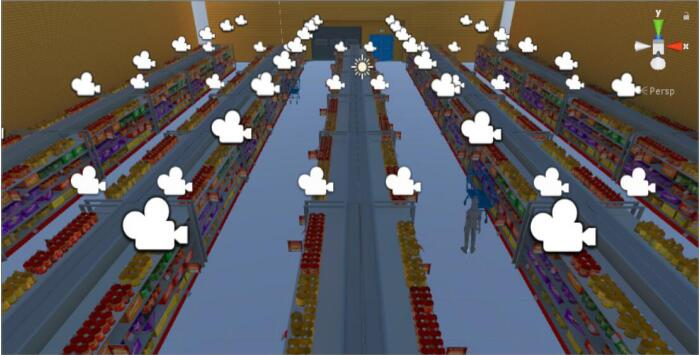
\includegraphics[width=7cm,scale=0.8]{supermarket.jpg}}
\caption{The whole simulated supermarket scene}
\label{fig}
\end{figure}

After setting up the scene, we also need to adjust the visual field and angle of each camera to get the best shooting pictures.
Through calculation and field investigation, we draw the h-fov is 1.2 bin is best for catching the maximum range and clearer picture, and the each camera can cover 2 bin.
In Fig.9, we can see the cameras which on shelves can clearly obtain the type and quantity of items, this provides a great help for our later identification.

\begin{figure}[htbp]
\centerline{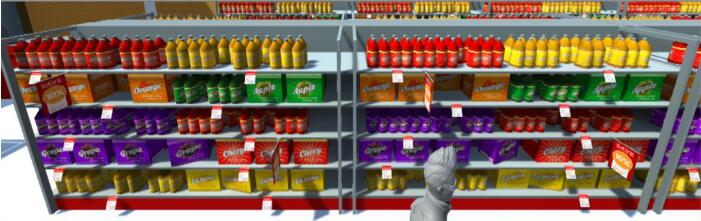
\includegraphics[width=7cm,scale=0.8]{shelves.jpg}}
\caption{Information on the shelf captured by camera shuttle}
\label{fig}
\end{figure}

The simulated scene is based on the real scene, it can serve as a reference.
In this scene, we can design the placement of cameras, and calculate the location of the camera in the real scene and the number of cameras needed.
Unity3D provide method of capturing each camera image, use the clear screenshot F9 to get the picture which is describe the items type and quantity on shelves, and it is resolution is 1600*1200.
Then use pictures what we get to do item recognition and identify their type and number, ultimately get the data for the all items, calculate what kind and quantity customers take away.

\subsection{Item Recognition}

After setting up the scene, we need to add an image recognition system to each camera in the scene.
As mentioned above, YOLOv3 is suitable for items image recognition, we will use this recognition method for items image processing.
The YOLOv3 depends on OpenCV3.40 and CUDA8.0, which are our tools for training and recognition.
There are other ways to train and recognize our data.
TensorFlow\cite{199317} is a free and open-source software library for dataflow and differentiable programming across a range of tasks, it can as well be used in computer vision processing.
In our simulation, OpenCV still is our main train and recognize, because it's easier to operate in our limited equipment.

In order to recognize the picture what we get for the scene's cameras, we have to pre-process the types of items and train them.
There are lots of goods pictures in the internet, then we selected 1000 representative types for us to train.
In order to make the simulation results closer to the real scene, the goods we selected were placed on the shelves and they were placed according to the way of the shopping mall.
After obtaining samples pictures, these pictures should be marked so that the system can remember their characteristics and what exactly item is.

\begin{figure}[htbp]
\centerline{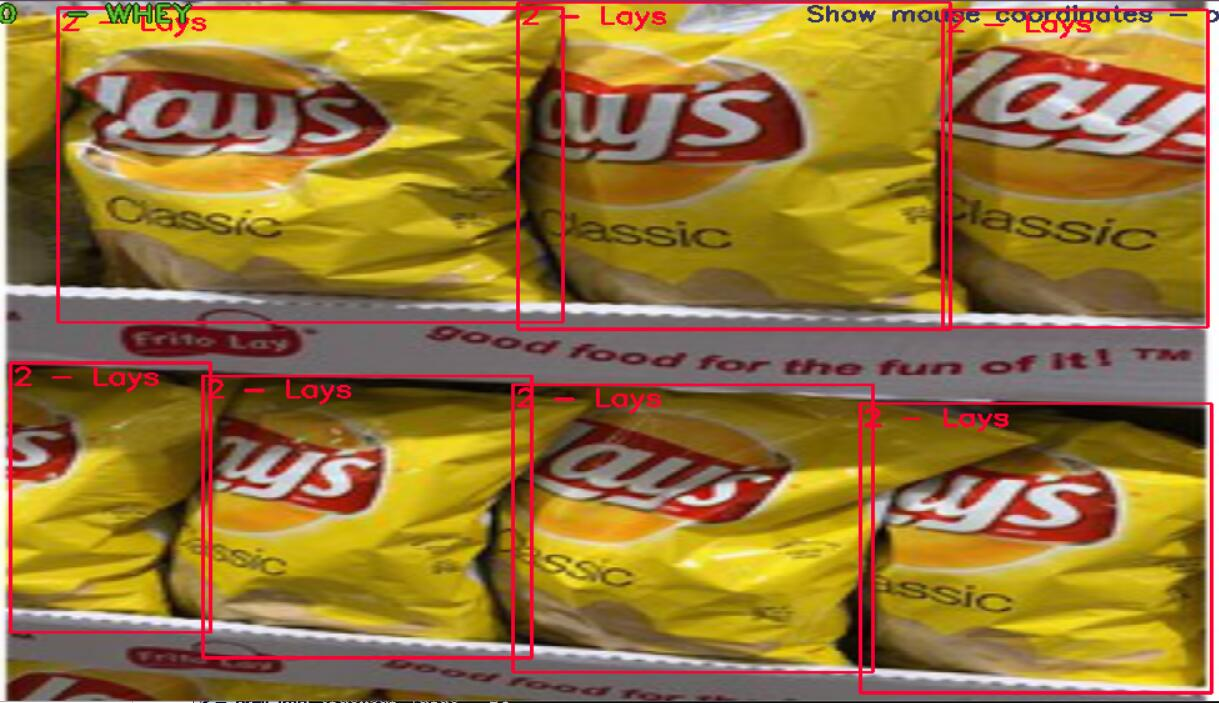
\includegraphics[width=7cm,scale=0.8]{LaysMarked.jpg}}
\caption{The test set image what we use in our experiment}
\label{fig}
\end{figure}

After marking all items, we will put all the pictures and data of the pictures into our pre-designed YOLO architecture for training.
The purpose of training is to get the weight of each item so that our system can distinguish their type and accurately judge when inputting new pictures.
In our simulator, we had 5,000 iterations of the data to get a lowest loss.
When all the data has been trained, new data can be allowed to enter.
We selected a picture that was not included in our data set to try the training results.
The category of this item is the one that has been trained by our system.
We searched the pictures of this item randomly on the Internet and put them into our system for identification.
The recognition result as shown in Fig.11

\begin{figure}[htbp]
\centerline{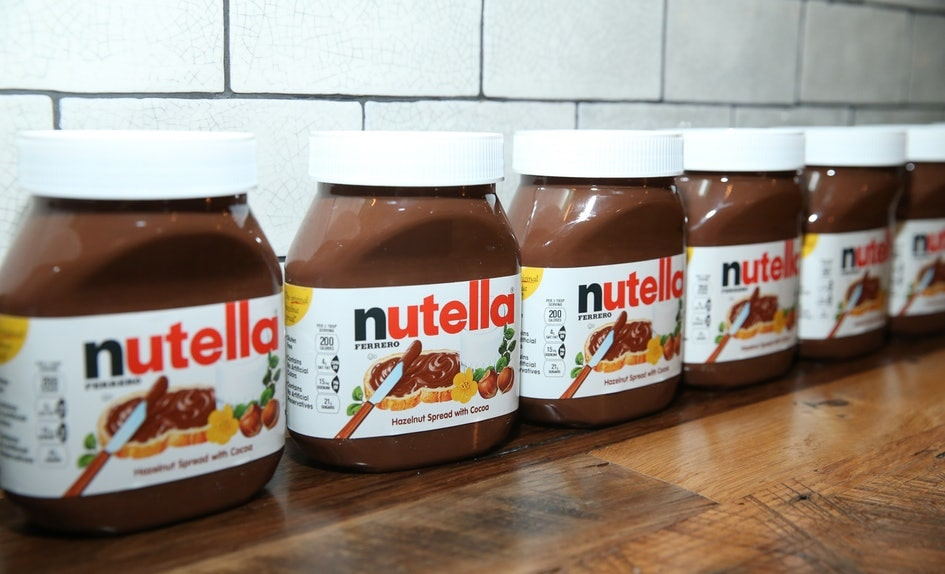
\includegraphics[width=3.5cm,scale=0.6]{nutella.jpg} 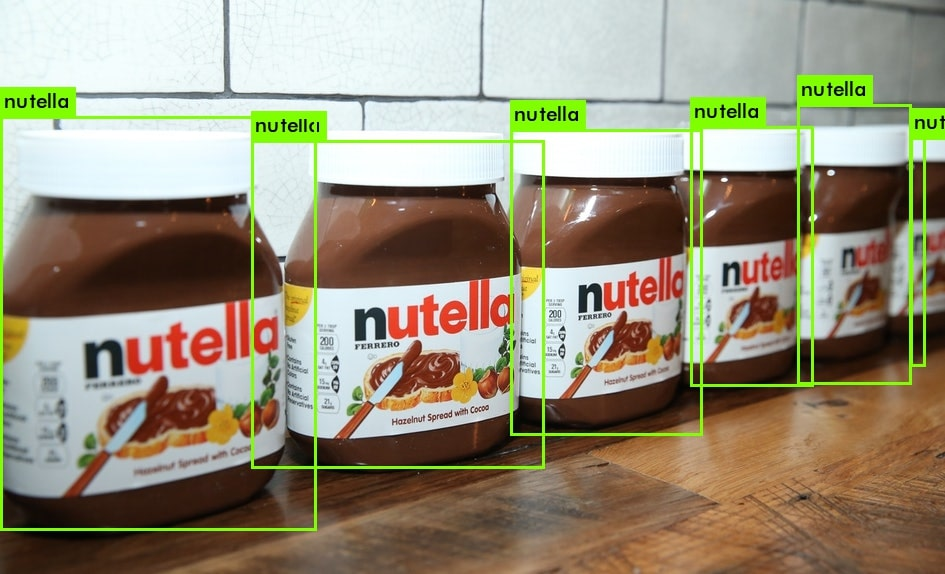
\includegraphics[width=3.5cm,scale=0.6]{nutella2.jpg}}
\caption{Put the "nutella" pictures into our recognition system and recognize the information.}
\label{fig}
\end{figure}

Our system can accurately identify the object and the number of objects in this picture, its recognition rate can reach 98\%.
This means that when the camera in the scene intercepts the picture and puts it into our system, it can accurately identify the type and number of them.
It shows that the system we built is feasible to be used in real scenes.
Ultimately we'll have it with multi cameras to achieve cashier-free supermarket.


